\section{Measurements and Tests}
% Laser: KY 008
% Photo Resistor: KY
The measurements and tests cover the power drain from the sensor, laser and the esp32l inlcuding deepsleep and bluetooth, to determine the optimal setup. The setup for the measurement or test is explained in each section. Again, the tests do not aim for scientific and statisitcal significance but as a guiding point. Their goal is to provide an order of magnitude of the power consumption of the individual components to guide future architectural decisions. 


\subsection{Laser}
We measured the laser on a power source directly connected to the esp32 which has an output rating of $4.695V$ with a max current of $80mA$. The laser consumed on average $25mA$ and thus the power consumption is
\begin{equation*}
    4.695V * 25mA = 0.117W
\end{equation*}
which is, as expected, fairly high. In a setup with to lasers per goal, this could be a realy problem


\subsection{Sensor}
Next, we measured the power consumption of the sensor, again powered by the esp32, so $4.695V$ with a max current of $80mA$. It consumed on average $3.5mA$ when the laser was hitting the sensor and $3.8mA$ when it was not. As the default state is hitting and only goals, so very short periods, are not hitting, the power consumption is
  \begin{equation*}
      4.695V * 3.5mA = 0.016W.
    \end{equation*}
This is inline with the expectations, as the resistance drops when the laser hits the sensor. 
To summarize, together the sensor and laser consume around  
\begin{equation*}
    0.016W + 0.117W = 0.133W
  \end{equation*}
in idle and a little bit more when a goal is scored. Thus the power consumption in one day is
\begin{equation*}
    0.133W * 24 = 3.19Whr
\end{equation*}
This is quite a lot especially running on a battery with only
\begin{equation*}
    0.133W * 24 = 12Whr
\end{equation*}

\subsection{ESP32 Modes}
The esp32 development board from wemos consumes around $43mA$ in idle and $0.128mA$ in deepsleep. This is much higher than esp32 wroom board which is supposed to only consume $20mA$ in idle and $0.01mA$ in deepsleep\cite{InsightI15esp32ModesWroom:online}. \Cref{fig:esp32Comp} shows both microcontrollers side by side. 

\begin{figure}[H!]
    \centering
    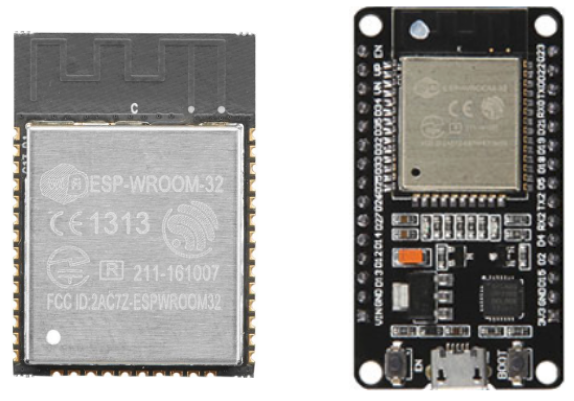
\includegraphics[scale=0.4]{figures/esp32-wroom-wemos.png}% picture filename
    \caption{ESP32 wroom (left) and Wemos development board.}\label{fig:esp32Comp}
\end{figure}

The development board has a microusb controller and many integrated circuits to prevent short circuits and other problems as well as over an LED, microUSB in and buttons for reseting and power of microUSB. All these extra components add up to the significant power consumption difference. For the production we will thus use esp32 wrooms and soldier the connections our selfs. So instead of using our numbers, we will use the numbers from the esp32 wroom controller.\\

The power consumption also changes during boot time and while bluetooth is active. In the former, the processor takes a lot of power, while in the latter it is the radio chip, including antenna. \\

In our tests waking up from deepsleep took around $300ms$ and increased current consumption to about $80mA$ \footnote{This was done via eye measurment with a lot of fluctations, so the numbers are really only approximates.}. Especially, the wake up time seems quite slow and we would like to test this further and search for wake up optimizations in further research.
During sending and receiving of data, the power consumption increased to $70mA$.\\

To summarize each wake up costs at least
\begin{equation*}
    80mA * 7V / 3600 * (3/10) = 12Whr
\end{equation*}




\subsection{BLE Tests}